\addtolength{\tabcolsep}{-4.5pt}    
% \setlength{\mywidth}{0.1932\textwidth}
\bgroup
\def\arraystretch{0.5}%  1 is the default. Controls vertical spacing.
\begin{figure}[th]
\small
\begin{tabular} {cc|cc}
Label & Style Image & Encoder1 & Encoder2
\\
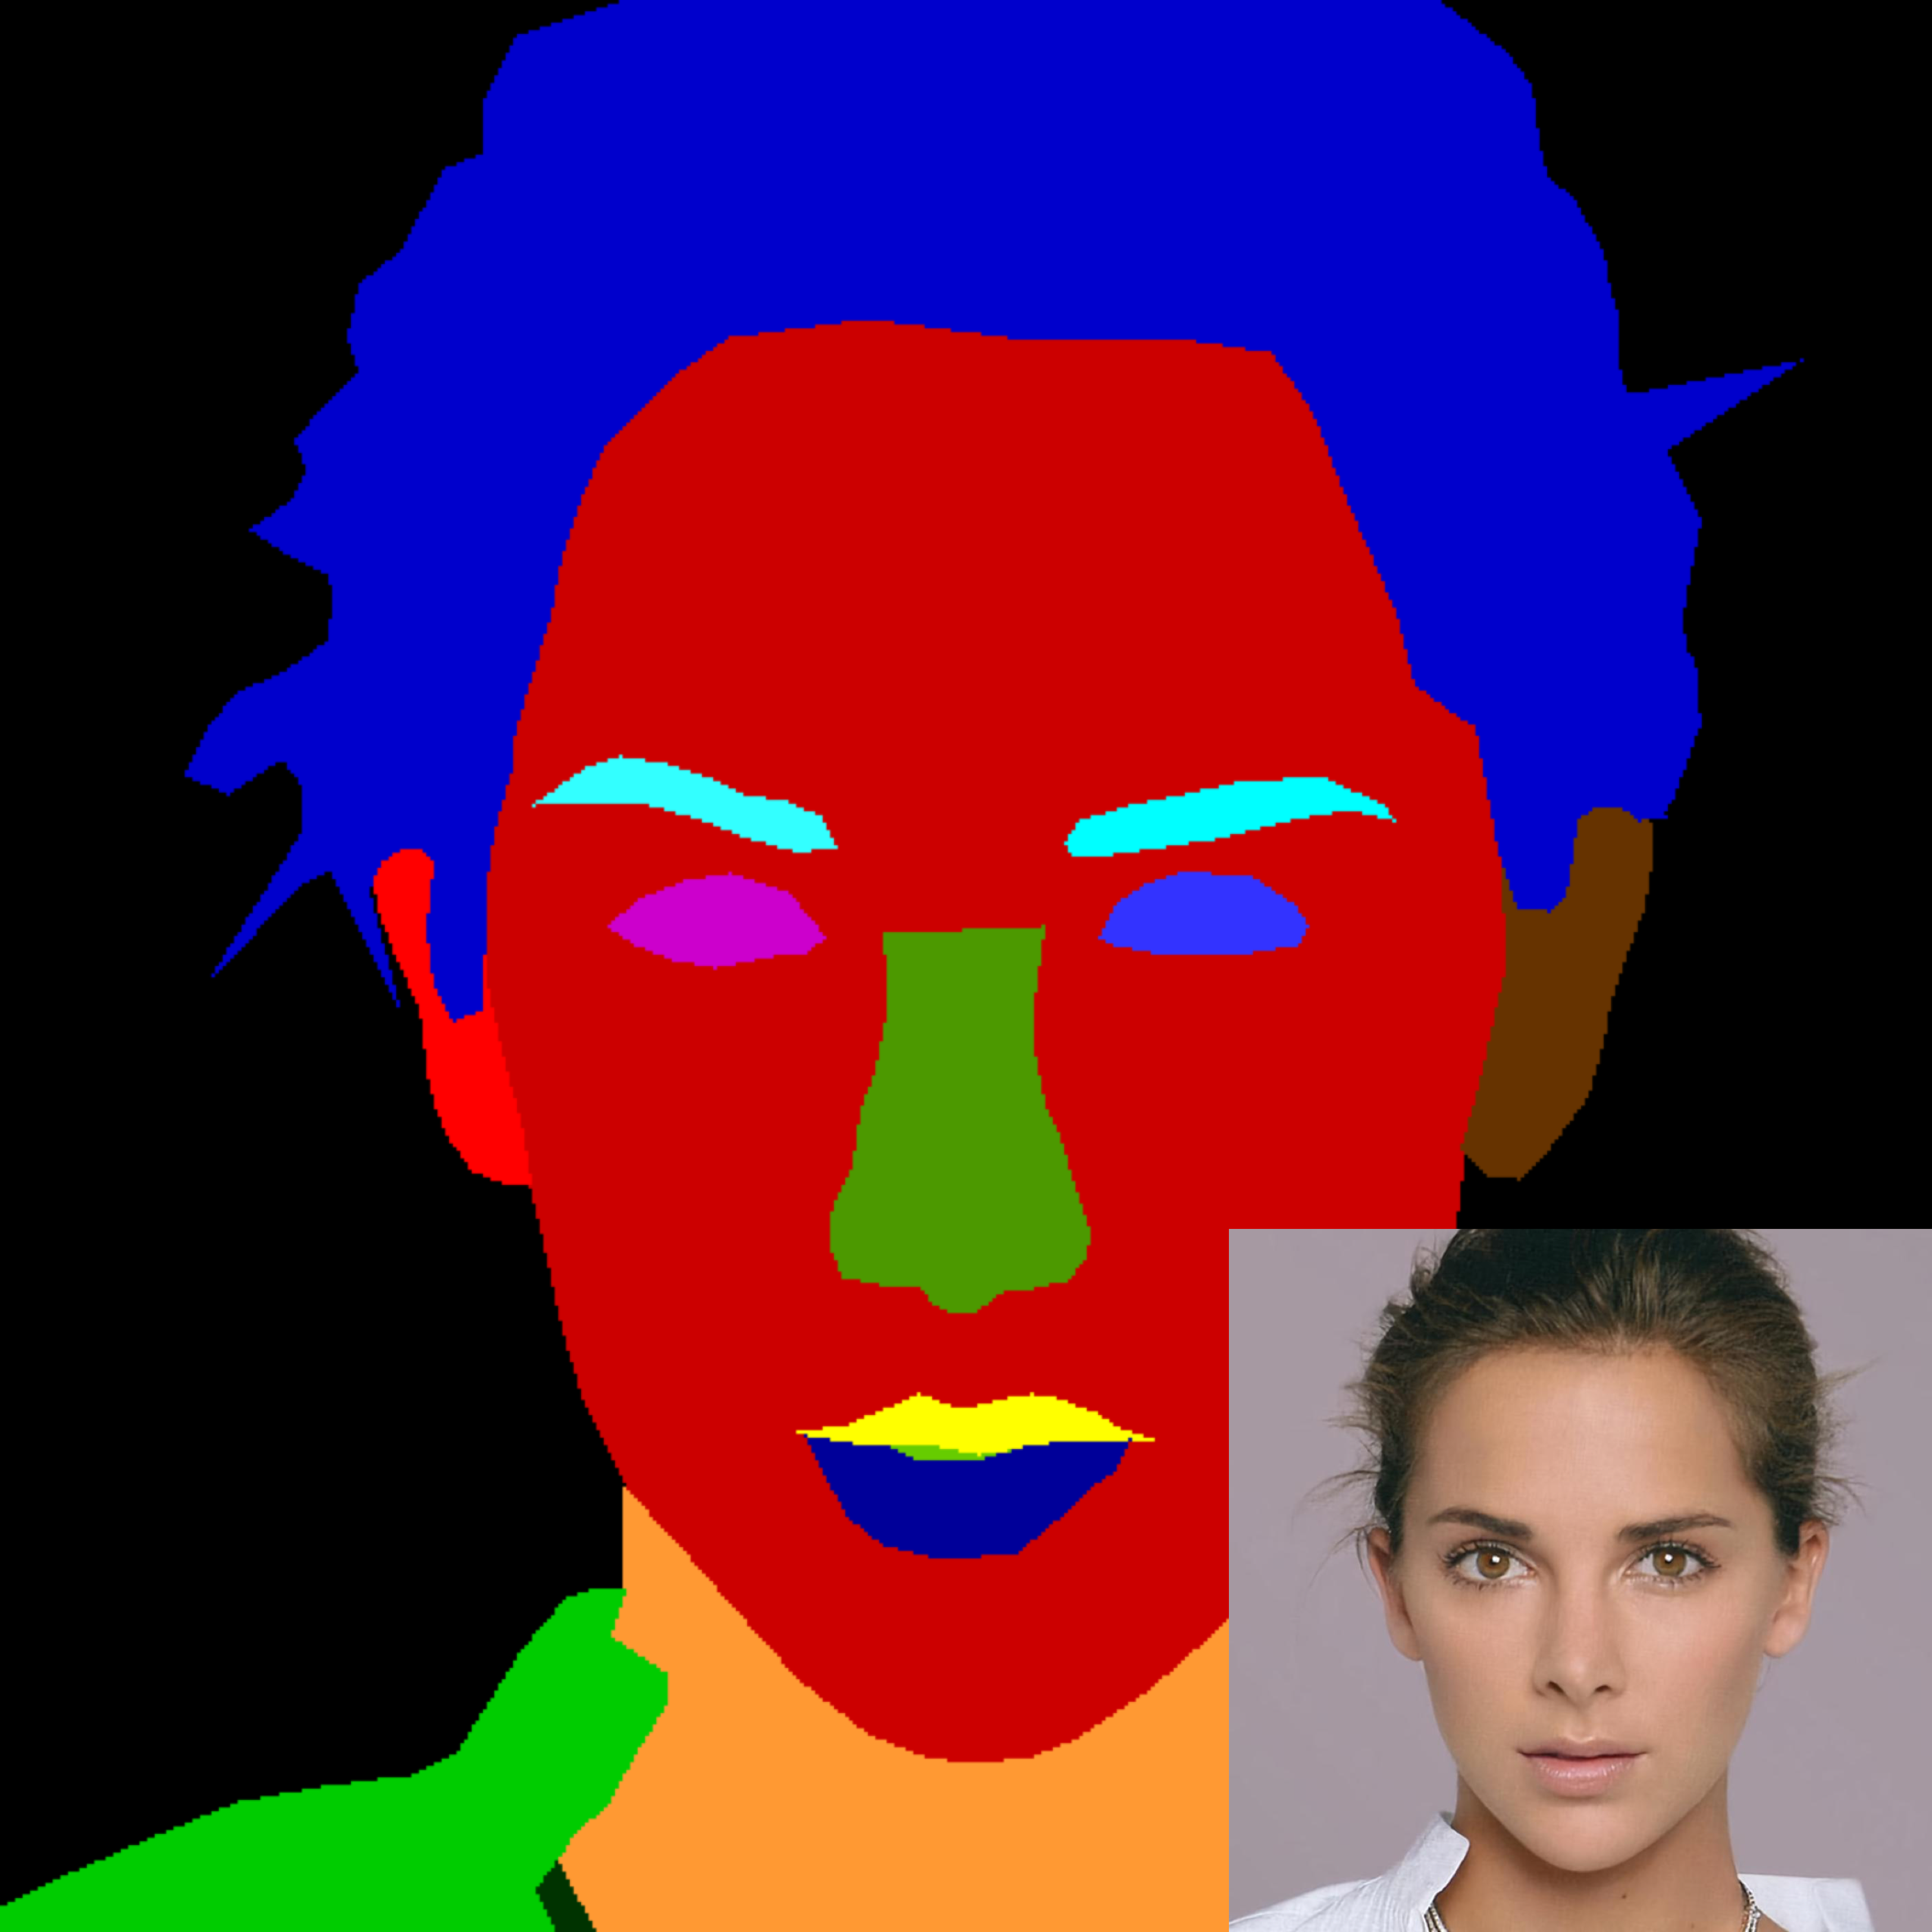
\includegraphics[width=0.11\textwidth]{Images/Encoder_search/encoder_1.png} & 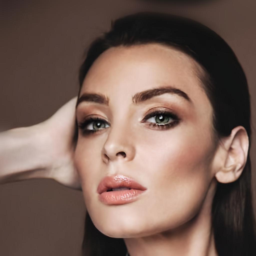
\includegraphics[width=0.11\textwidth]{Images/Encoder_search/style/29659.png} &
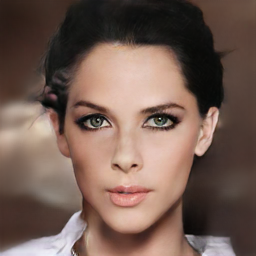
\includegraphics[width=0.11\textwidth]{Images/Encoder_search/SEAN_level/1.png} &   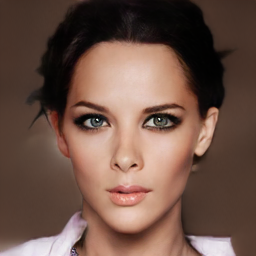
\includegraphics[width=0.11\textwidth]{Images/Encoder_search/Unified/1.png}\\ 

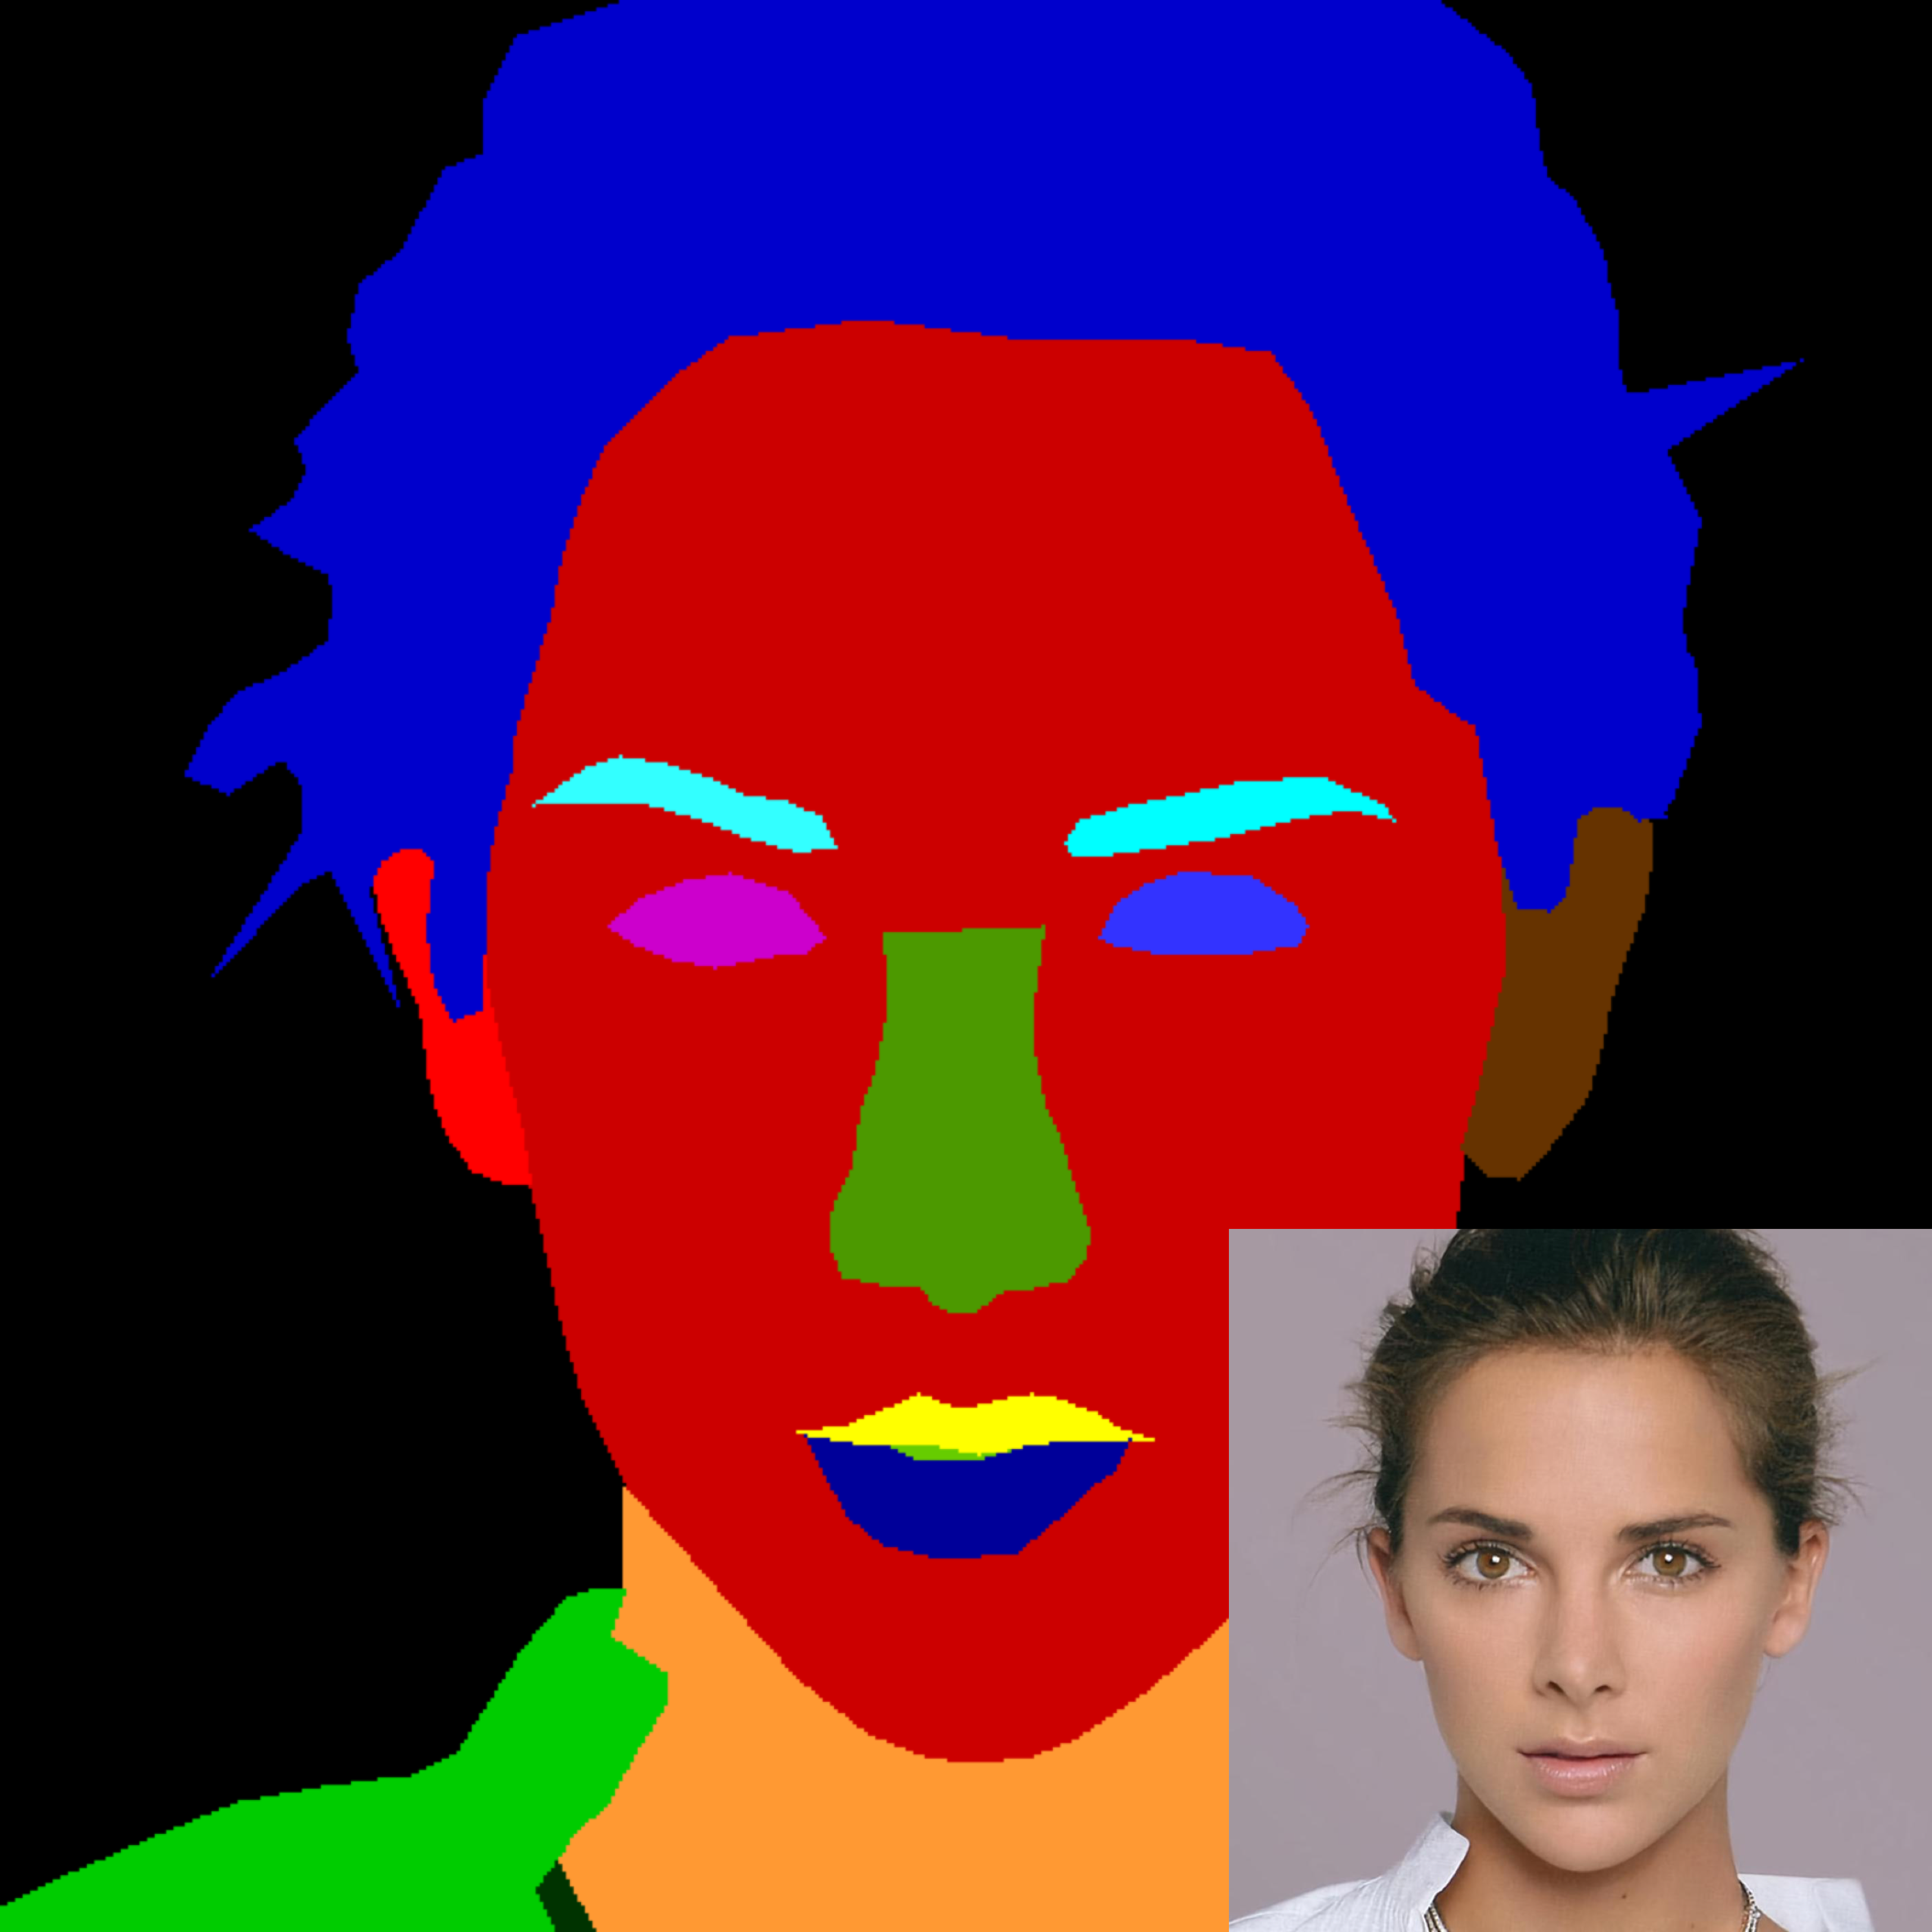
\includegraphics[width=0.11\textwidth]{Images/Encoder_search/encoder_1.png} & 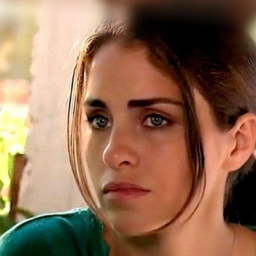
\includegraphics[width=0.11\textwidth]{Images/Encoder_search/style/29598.png} &
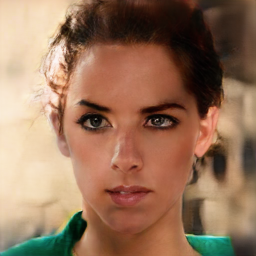
\includegraphics[width=0.11\textwidth]{Images/Encoder_search/SEAN_level/2.png} &   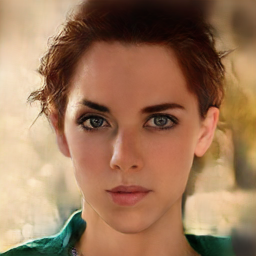
\includegraphics[width=0.11\textwidth]{Images/Encoder_search/Unified/2.png}\\ 

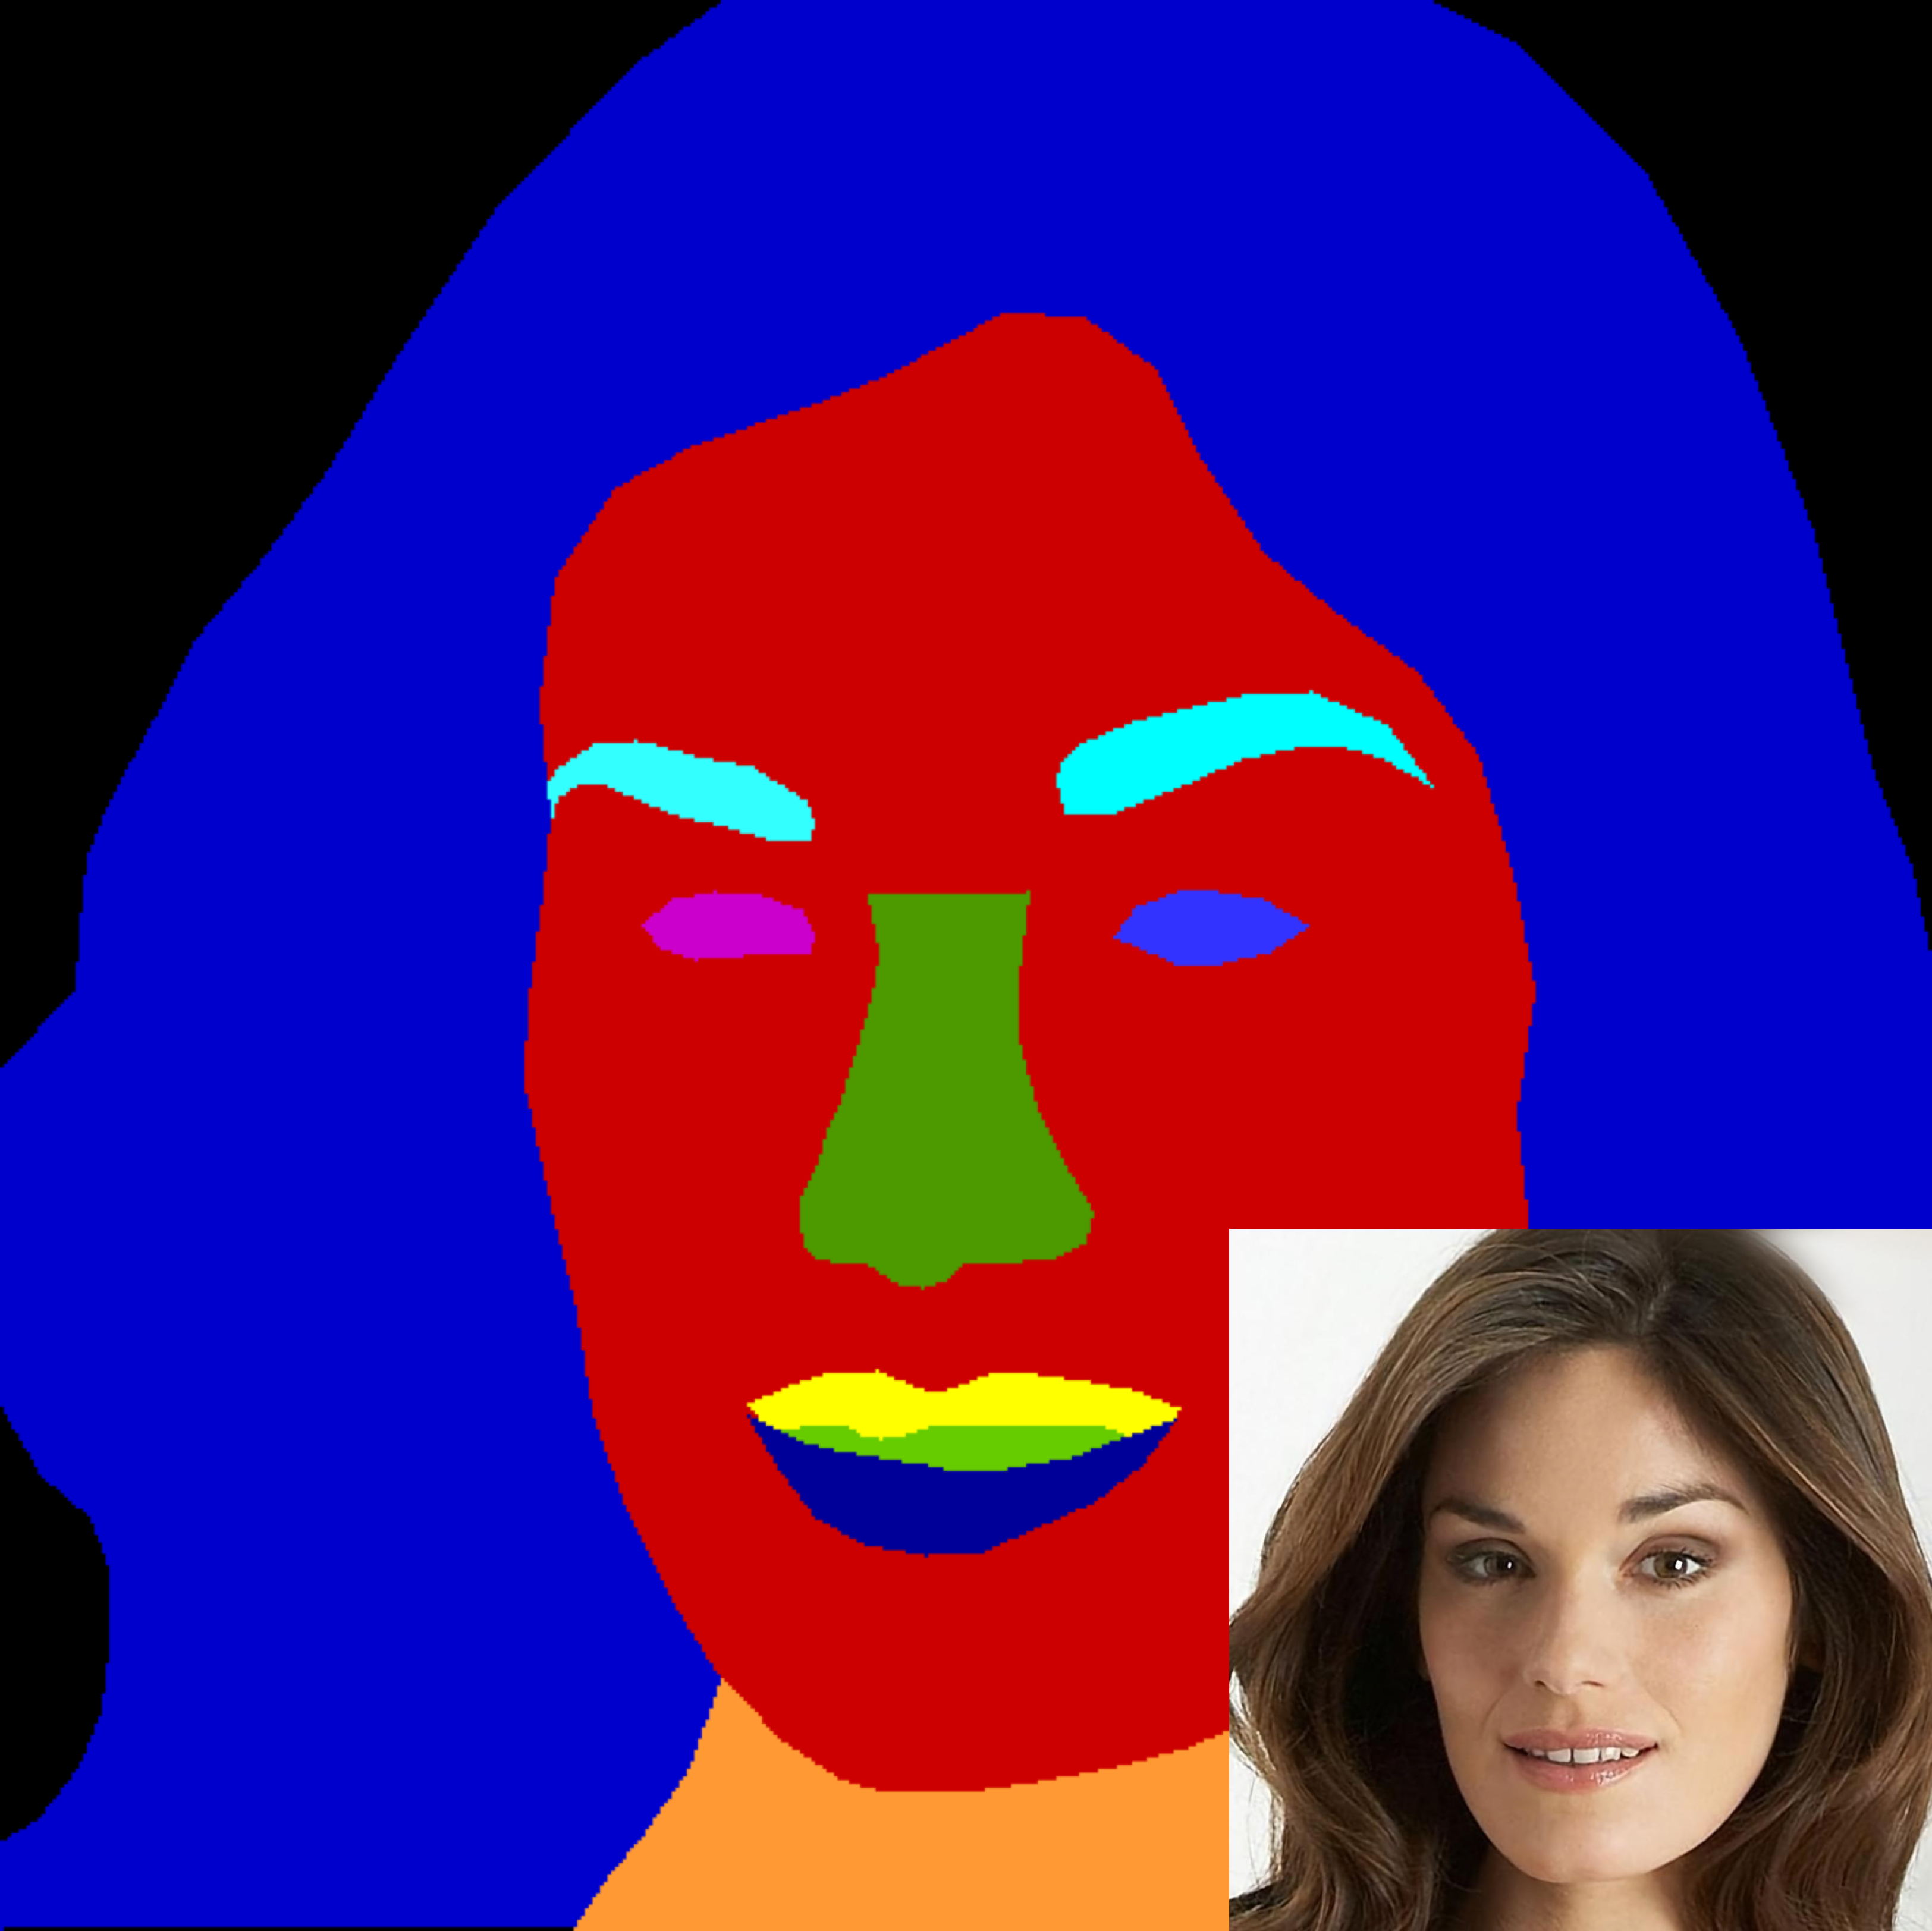
\includegraphics[width=0.11\textwidth]{Images/Encoder_search/encoder_2.png} & 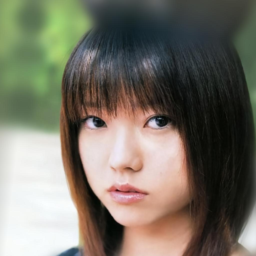
\includegraphics[width=0.11\textwidth]{Images/Encoder_search/style/29573.png} &
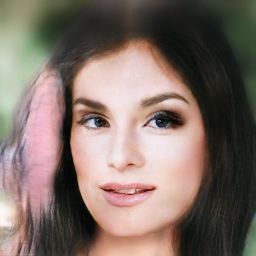
\includegraphics[width=0.11\textwidth]{Images/Encoder_search/SEAN_level/3.png} &   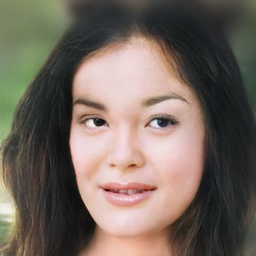
\includegraphics[width=0.11\textwidth]{Images/Encoder_search/Unified/3.png}\\ 

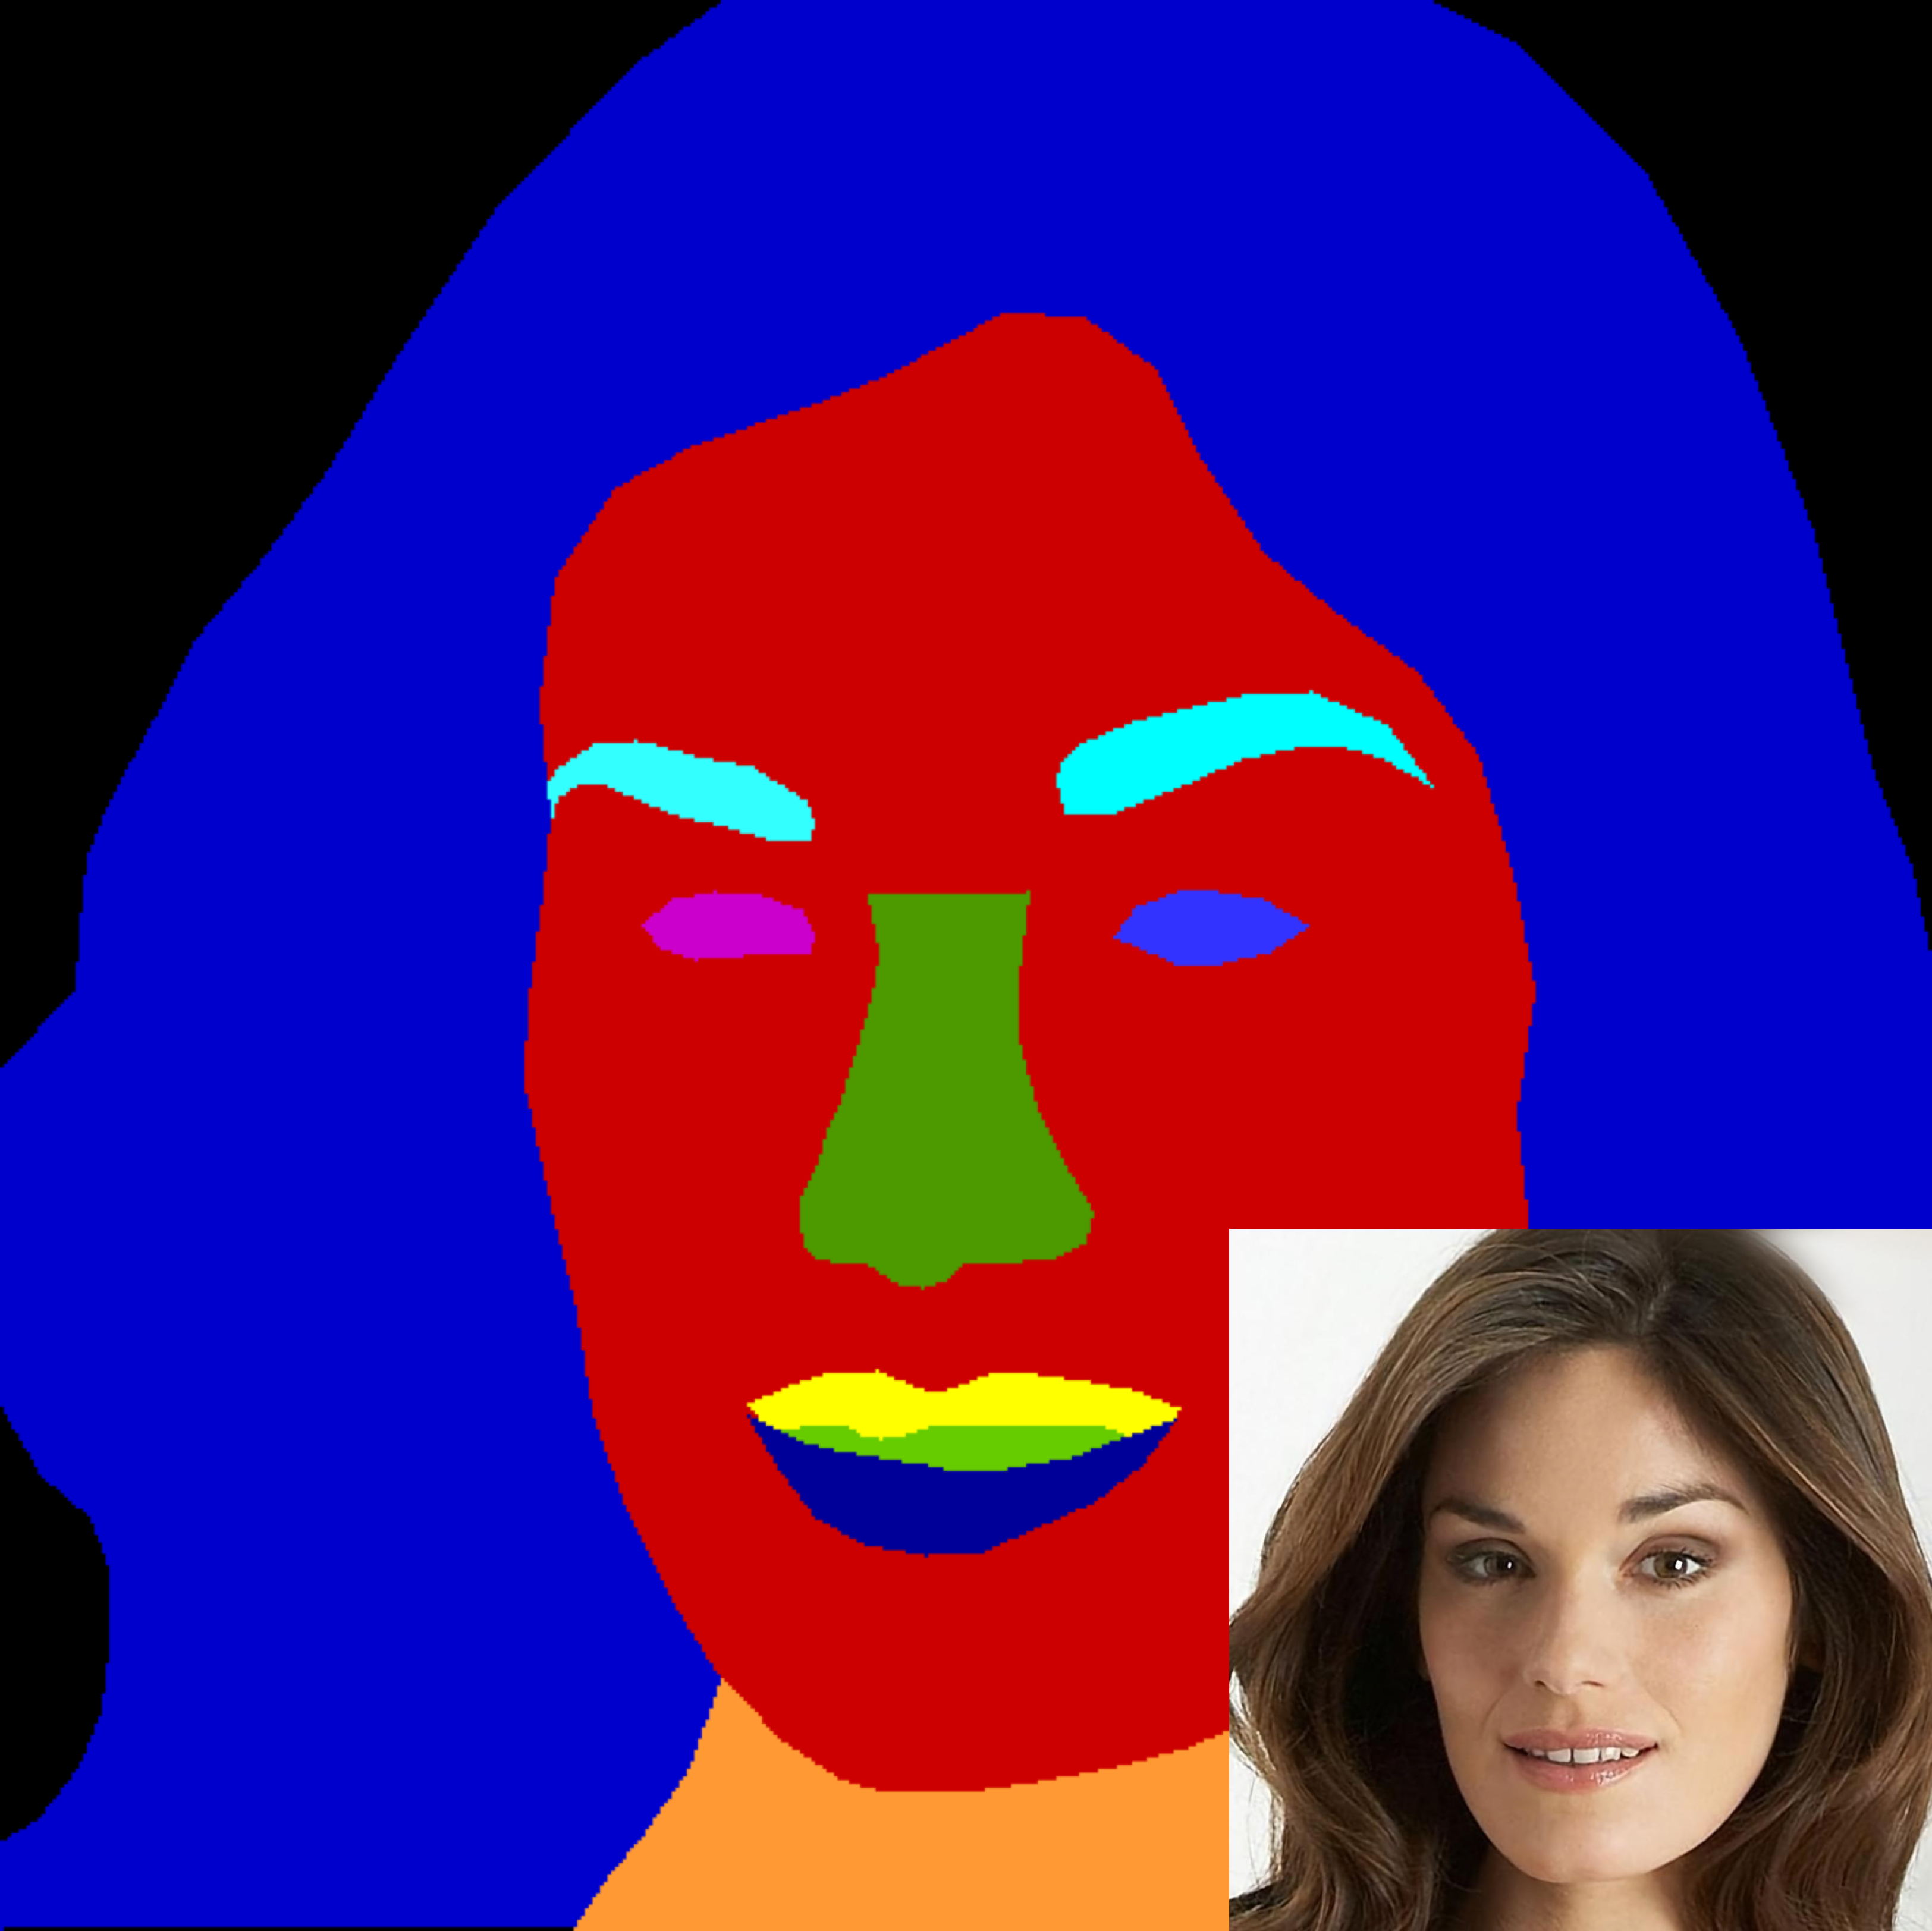
\includegraphics[width=0.11\textwidth]{Images/Encoder_search/encoder_2.png} & 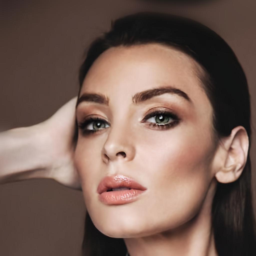
\includegraphics[width=0.11\textwidth]{Images/Encoder_search/style/29659.png} &
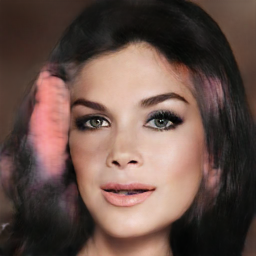
\includegraphics[width=0.11\textwidth]{Images/Encoder_search/SEAN_level/4.png} &   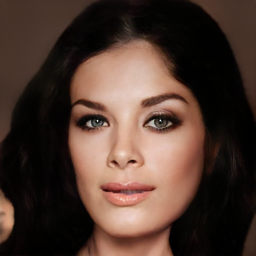
\includegraphics[width=0.11\textwidth]{Images/Encoder_search/Unified/4.png}\\ 


\end{tabular}
\vspace{-2mm}
	\caption{Encoder choice justification. Encoder1 is the SEAN-level encoder and Encoder2 is the unified encoder. SEAN-level encoder is more sensitive to the poses and unlabeled parts of the style image due to the overfitting. Using unified encoder can get more robust style transfer results.}
	\label{fig:Encoder Comparison}	
\vspace{-3mm}	
 \end{figure}
 \egroup
 \addtolength{\tabcolsep}{4.5pt}